\documentclass[a4paper]{article}

\usepackage[default]{lato}
\usepackage[swedish]{babel}
\usepackage[dvipsnames]{xcolor}
\usepackage[T1]{fontenc}
\usepackage[utf8]{inputenc}
\usepackage{graphicx}
\usepackage{fancyhdr}
\usepackage{lastpage}
\usepackage{parskip}

\definecolor{cerise}{RGB}{232, 61, 132}
\definecolor{gray3}{RGB}{66, 66, 66}

\addtolength{\textheight}{4cm}
\addtolength{\voffset}{-2cm}
\addtolength{\textwidth}{2cm}
\addtolength{\hoffset}{-1cm}
\setlength{\headheight}{40pt}

\pagestyle{fancy}
\thispagestyle{fancy}
\fancyhead[L]{\small{
    Motion till Val-SM % Skriv SM-namn
\\\textcolor{gray3}{
    15-03-2023 % Datum för SM
}}}
\fancyhead[C]{\includegraphics[width=1.25cm,height=1.25cm]{./skold-color.pdf}}
\fancyhead[R]{\small{\textcolor{gray3}{
    Erik Hedlund\\ % Skriv ditt namn här
    sida \thepage{} av \pageref{LastPage}}}}
\fancyfoot[C]{\small{\textcolor{gray3}{Konglig Datasektionen, THS 100 44, datasektionen.se}}}
\renewcommand{\headrulewidth}{0pt}

\title{\textcolor{cerise}{\textbf{
    Motion angående\\
    Förbudget för METAspexet 2024
}}}

\date{}

\begin{document}

\maketitle
\thispagestyle{fancy} % Smutsigt fulhack för att få header på första sidan

\section*{\textcolor{cerise}{
    Bakgrund
}}

Ni vet vad man säger? Nytt år, nytt spex, och som den sanningen lyder så kommer det just ett METAspexet 2024 nästa år också, vilken grej!

Men med det här nya spexet kommer det ju behövas en ny teater, och tänka sig, det har METAspexet 2023 redan fixat till METAspexet 2024.
Något som saknas för denna teater dock är en budget och därför skulle vi vilja spika poster för lokalhyra och biljettintäkter redan det här SM:et,
då teaterkontraktet redan är påskrivet.

Ytterligare hade spexet en uppstartshelg för chefsgruppen på Osqvik ifjol med ett gäng kortare utbildningar varvat med lite gött häng. Det är något
vi gärna skulle ha nästkommande spexår också, och har därför slängt in dem budgetposterna i den här motionen också.

\textbf{TL:DR Spexet 2024 har verksamhet innan dess budget läggs på Budget-SM och därför lägger vi en ``förbudget''. Räkna inte med att METAspexet 2024:as slutgiltiga budget lär vara plus budgeterat...}

\section*{\textcolor{cerise}{
    Förslag till beslut
}}

	Mot bakgrund av ovanstående yrkar jag:

\newcounter{attnummer}
\setcounter{attnummer}{1}
\begin{list}{\bf att$_{\theattnummer}$\stepcounter{attnummer}}{}
\item Den bifogade budgeten för METAspexet 2024 antas i sin helhet
\end{list}

\vspace{2cm}
\noindent
% Name, eventuell titel eller annat skoj
Erik Hedlund \& Jakob Carlsson, Direqteurer 2023

% Avkommentera följande om du vill visa en bild
\begin{center}
 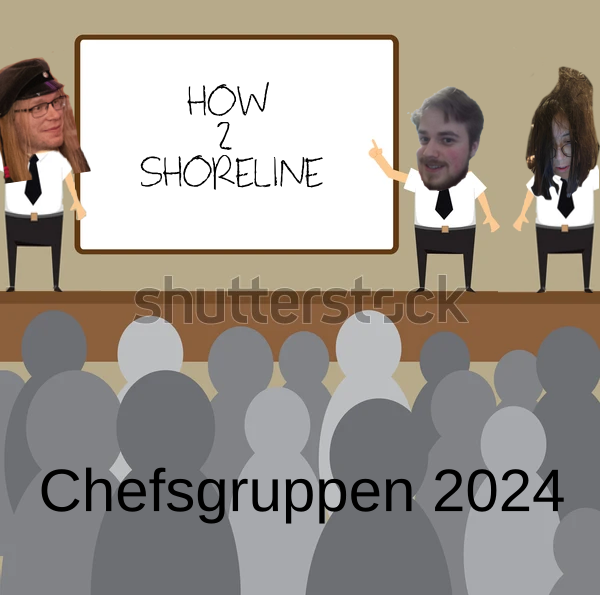
\includegraphics[scale=0.5]{
    % Eventuell fin bild du vill visa.
     ./lecture.png
 }
\end{center}


\end{document}
